\documentclass{article}
\usepackage[utf8]{inputenc}
\usepackage{my_preamble}


\title{Microeconomics Diagrams}
\author{Joel Pointon}
\date{June 2020}

\begin{document}
\maketitle
All graphs in this document were created by Joel Pointon and can be found on \href{https://github.com/pointonjoel/TeXonomics}{GitHub}. Note that graphs are displayed in alphabetical order.

\listoffigures

\begin{figure}[H]
    \centering
    \documentclass[class=article, crop=false]{standalone}
\usepackage{my_preamble}
\begin{document}
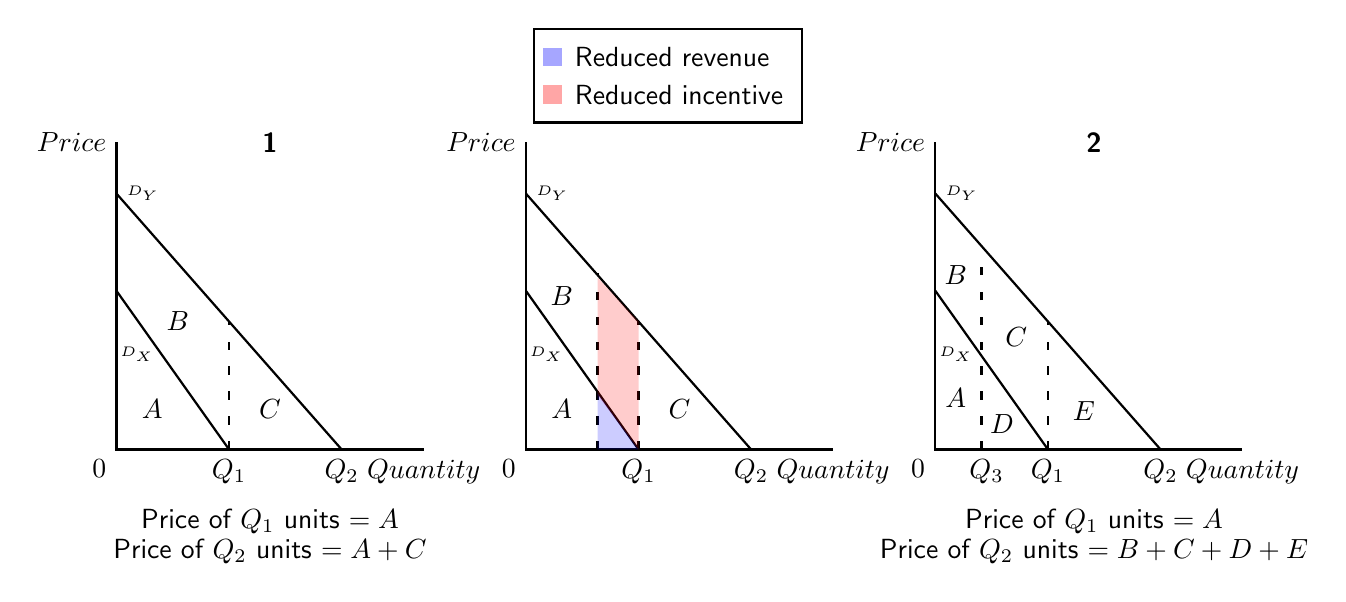
\begin{tikzpicture}[thick,font=\sffamily,scale=1.3,
  					bluenode/.style={shape=rectangle, fill=blue!35, line width=2},
  					rednode/.style={shape=rectangle, fill=red!35, line width=2}
					]
	%axies
	\draw (-6,3) node[left]{$Price$} -- (-6,0) node[below left] {$0$} -- (-3,0) node[below]{$Quantity$}; %panel a (1)
	\draw (-2,3) node[left]{$Price$} -- (-2,0) node[below left] {$0$} -- (1,0) node[below]{$Quantity$}; %panel b
	\draw (2,3) node[left]{$Price$} -- (2,0) node[below left] {$0$} -- (5,0) node[below]{$Quantity$}; %panel c (2)
	  
	 %Panel a-----------------------------------------------
	\draw[] (-6,2.5) -- (-3.8,0); %demand y
	\node[right] at (-6,2.5) {\tiny{$D_{Y}$}}; %Y's Demand label
	\draw[] (-6,1.55) -- (-4.9,0); %demand x
	\node[below] at (-5.8,1.1) {\tiny{$D_{X}$}}; %X's Demand label
	\draw[loosely dashed] (-4.9,0) -- (-4.9,1.25); %separator
	\node[] at (-5.65,0.4) {$A$}; %A label
	\node[] at (-5.4,1.25) {$B$}; %B label
	\node[] at (-4.5,0.4) {$C$}; %C label
	\node[below] at (-4.9,0) {$Q_{1}$}; %Q1 label
	\node[below] at (-3.8,0) {$Q_{2}$}; %Q2 label
		
	 %Panel b-----------------------------------------------
	\draw[] (-2,2.5) -- (0.2,0); %demand y
	\node[right] at (-2,2.5) {\tiny{$D_{Y}$}}; %Y's Demand label
	\draw[] (-2,1.55) -- (-0.9,0); %demand x
	\node[below] at (-1.8,1.1) {\tiny{$D_{X}$}}; %X's Demand label
	\draw[loosely dashed] (-0.9,0) -- (-0.9,1.25); %separator 1
	\draw[loosely dashed] (-1.3,0) -- (-1.3,1.72); %separator 2
	\node[] at (-1.65,0.4) {$A$}; %A label
	\node[] at (-1.65,1.5) {$B$}; %B label
	\node[] at (-.5,0.4) {$C$}; %C label
	\node[below] at (-0.9,0) {$Q_{1}$}; %Q1 label
	\node[below] at (0.2,0) {$Q_{2}$}; %Q2 label	
	
	\fill [fill=red, fill opacity=0.2] (-0.9,0) node[left]{} -- (-0.9,1.25) node[below left] {} -- (-1.3,1.68) node[below left] {} -- (-1.3,0.53) node[below left] {}; %fill
	\fill [fill=blue, fill opacity=0.2] (-0.9,0) node[left]{} -- (-1.3,0) node[below left] {} -- (-1.3,0.55) node[below left] {}; %fill 
	
	 %Panel c-----------------------------------------------
	\draw[] (2,2.5) -- (4.2,0); %demand y
	\node[right] at (2,2.5) {\tiny{$D_{Y}$}}; %Y's Demand label
	\draw[] (2,1.55) -- (3.1,0); %demand x
	\node[below] at (2.2,1.1) {\tiny{$D_{X}$}}; %X's Demand label
	\draw[loosely dashed] (3.1,0) -- (3.1,1.25); %separator 1
	\draw[loosely dashed] (2.45,0) -- (2.45,1.9); %separator 2
	\node[] at (2.2,0.5) {$A$}; %A label
	\node[] at (2.2,1.7) {$B$}; %B label
	\node[] at (2.79,1.1) {$C$}; %C label
	\node[] at (2.65,0.25) {$D$}; %D label
	\node[] at (3.45,0.38) {$E$}; %E label
	\node[below] at (3.1,0) {$Q_{1}$}; %Q1 label
	\node[below] at (4.2,0) {$Q_{2}$}; %Q2 label
	\node[below] at (2.5,0) {$Q_{3}$}; %Q3 label		
	
	%extras--------------------------------------------------
	%legend
	\matrix [draw,above] at (current bounding box.north) {
  	\node [bluenode,label=right:Reduced revenue] {}; \\
  	\node [rednode,label=right:Reduced incentive] {}; \\
};	
	%panel titles
	\node[] at (-4.5,3) {\textbf{1}}; %Panel 1 label
	\node[] at (3.55,3) {\textbf{2}}; %Panel 2 label

	%descriptions
	\node[] at (3.55,-0.7) {Price of $Q_{1}$ units $= A$}; %Q1 price
	\node[] at (3.55,-1) {Price of $Q_{2}$ units $= B+C+D+E$}; %Q2 price
	\node[] at (-4.5,-0.7) {Price of $Q_{1}$ units $= A$}; %Q1 price
	\node[] at (-4.5,-1) {Price of $Q_{2}$ units $= A+C$}; %Q2 price
\end{tikzpicture}
To make them indifferent between plan $Q_{1}$ and $Q_{2}$ in graph 1, the firm must offer the prices above, leading to a CS of B. This is assuming that, if indifferent, the lower D will choose $Q_{1}$ and the higher D will choose $Q_{2}$. For panel 2, the firm offers $Q_{3}$ units (note $Q_{3}<Q_{1}$) and $Q_{2}$ units at the prices above. Here, there CS is reduced at B which is less than the area of B in panel 1.
\end{document}
    \caption{Second degree price discrimination}
    \label{fig:1}
\end{figure}
\begin{figure}[H]
    \centering
    \documentclass[class=article, crop=false]{standalone}
\usepackage{my_preamble}
\begin{document}
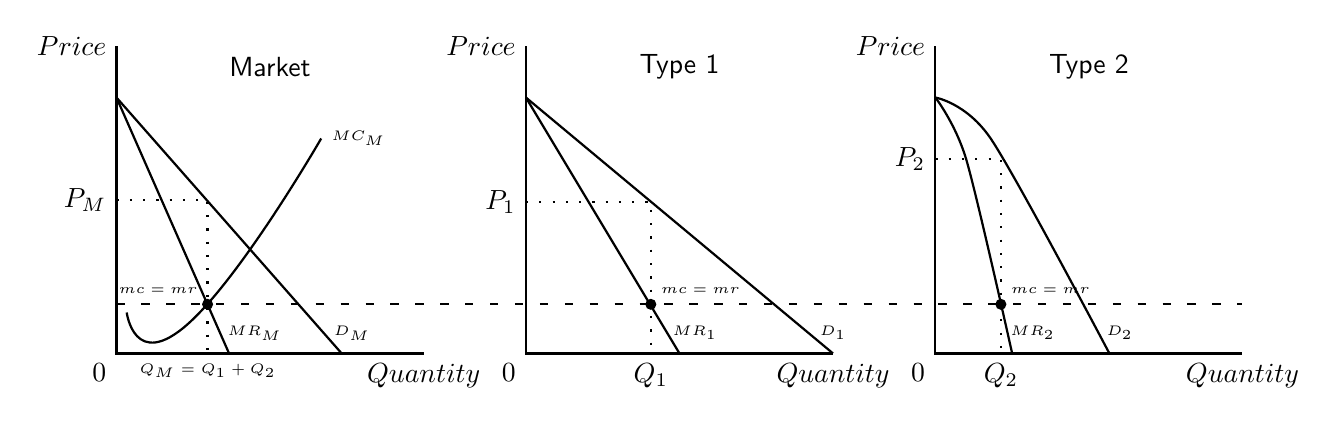
\begin{tikzpicture}[thick,font=\sffamily,scale=1.3]
	%axies
	\draw (-6,3) node[left]{$Price$} -- (-6,0) node[below left] {$0$} -- (-3,0) node[below]{$Quantity$}; %market
	\draw (-2,3) node[left]{$Price$} -- (-2,0) node[below left] {$0$} -- (1,0) node[below]{$Quantity$}; %type 1
	\draw (2,3) node[left]{$Price$} -- (2,0) node[below left] {$0$} -- (5,0) node[below]{$Quantity$}; %type 2
	
	%titles
	\node[] at (-4.5,2.8) {Market}; %Market title
	\node[] at (-0.5,2.8) {Type 1}; %Type 1 title
	\node[] at (3.5,2.8) {Type 2}; %Market title
	  
	 %market-----------------------------------------------
	\draw[] (-6,2.5) -- (-3.8,0); %demand
		\node[] at (-3.7,0.2) {\tiny{$D_{M}$}}; %Demand label
	\draw[] (-6,2.5) -- (-4.9,0); %mr
	\node[] at (-4.65,0.2) {\tiny{$MR_{M}$}}; %MR label
	\draw[] plot [smooth, tension=1] coordinates {(-5.9,0.4) (-5.3,0.29) (-4,2.1)}; %mc
	\node[right] at (-4,2.1) {\tiny{$MC_{M}$}}; %MC label
	\node[style={fill=black,circle,inner sep=0pt,minimum size=4pt}] at (-5.11,0.48) { }; %mc=mr node
	\node[above left]at (-5.11,0.48) {\tiny{$mc=mr$}}; %mc=mr label
	\draw[loosely dashed] (-6,0.48) -- (5,0.48); %mc line
	\draw[loosely dotted] (-6,1.5) node[left]{$P_{M}$} -| node[pos=0.25,below=3mm] {} (-5.11,0) node[below]{\tiny{$Q_{M}=Q_{1}+Q_{2}$}}; %dotted lines
	
	 %Type 1 - elastic-------------------------------------
	\draw[] (-2,2.5) -- (1,0); %demand
	\node[] at (1,0.2) {\tiny{$D_{1}$}}; %Demand1 label
	\draw[] (-2,2.5) -- (-0.5,0); %mr
	\node[] at (-0.35,0.2) {\tiny{$MR_{1}$}}; %MR1 label
	\node[style={fill=black,circle,inner sep=0pt,minimum size=4pt}] at (-0.78,0.48) { }; %mc=mr node
	\node[above right]at (-0.78,0.48) {\tiny{$mc=mr$}}; %mc=mr label	
	\draw[loosely dotted] (-2,1.48) node[left]{$P_{1}$} -| node[pos=0.25,below=3mm] {} (-0.78,0) node[below]{$Q_{1}$}; %dotted lines
	 
	 %Type 2 - inelastic------------------------------------
	%\draw[] (2,2.5) -- (3.5,0); %demand
	%\draw[] (2,2.5) -- (2.75,0); %mr
	\draw[] plot [smooth, tension=0.5] coordinates {(2,2.5) (2.54,2.1) (3.7,0)}; %demand
	\node[] at (3.8,0.2) {\tiny{$D_{2}$}}; %Demand2 label
	\draw[] plot [smooth, tension=0.5] coordinates {(2,2.5) (2.3,1.9) (2.75,0)}; %mr
	\node[] at (2.95,0.2) {\tiny{$MR_{2}$}}; %MR2 label
	\node[style={fill=black,circle,inner sep=0pt,minimum size=4pt}] at (2.64,0.48) { }; %mc=mr node
	\node[above right]at (2.64,0.48) {\tiny{$mc=mr$}}; %mc=mr label
	\draw[loosely dotted] (2,1.9) node[left]{$P_{2}$} -| node[pos=0.25,below=3mm] {} (2.64,0) node[below]{$Q_{2}$}; %dotted lines
\end{tikzpicture}
\end{document}
    \caption{Third degree price discrimination and the optimum bundles for the firm}
    \label{fig:2}
\end{figure}
\begin{figure}[H]
    \centering
    \documentclass[class=article, crop=false]{standalone}
\usepackage{my_preamble}
\begin{document}
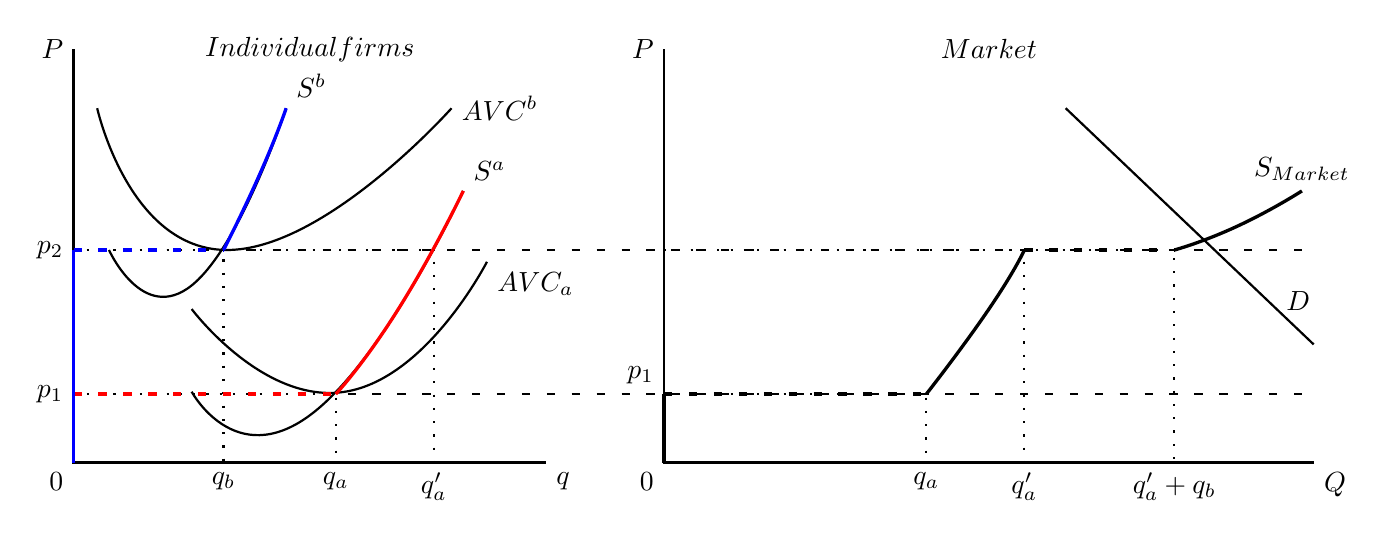
\begin{tikzpicture}[thick,font=\sffamily,scale=1.5]
	%axis and labels----------------------------
	 \draw (0,3.5) node[left]{$P$} -- (0,0) node[below left] {$0$} -- (4,0) node[below right]{$q$};
	   \draw (5,3.5) node[left]{$P$} -- (5,0) node[below left] {$0$} -- (10.5,0) node[below right]{$Q$};
	   \node[] at (2,3.5) {$Individual firms$}; %Firm label  
	   \node[] at (7.75,3.5) {$Market$}; %Market label  
	%Firm--------------------------------------
		%graphs	
		\draw[] plot [smooth, tension=1] coordinates {(1,1.3) (2.3,0.6) (3.5,1.7)}; %AVCa
		\draw[] plot [smooth, tension=1] coordinates {(1,0.6) (2,0.4) (3.3,2.3)}; %MCa
		\draw[] plot [smooth, tension=1] coordinates {(0.2,3) (1.3,1.8) (3.2,3)}; %AVCb
		\draw[] plot [smooth, tension=1] coordinates {(0.3,1.8) (1,1.5) (1.8,3)}; %MCb
		
		%dotted lines
		\draw[loosely dotted] (0,0.58) node[left]{$p_{1}$} -| node[pos=0.25,below=3mm] {} (2.22,0) node[below]{$q_{a}$}; %Dotted lines a1
		\draw[loosely dotted] (0,1.8) node[left]{} -| node[pos=0.25,below=3mm] {} (3.05,0) node[below]{$q^{\prime}_{a}$}; %Dotted lines a2
		\draw[loosely dashed] (0,0.58) -- (10.5,0.58); %p line
		\draw[loosely dotted] (0,1.8) node[left]{$p_{2}$} -| node[pos=0.25,below=3mm] {} (1.27,0) node[below]{$q_{b}$}; %Dotted lines b
		\draw[loosely dashed] (0,1.8) -- (10.5,1.8); %p line
		
		%Firm a supply curve	
		\draw[very thick, red] (0,0) -- (0,0.58); %part 1
		\draw[very thick, red, loosely dashed] (0,0.58)--(2.22, 0.58); %part 2
		\draw[very thick, red] plot [smooth, tension=1] coordinates{(2.22, 0.58) (2.75,1.3) (3.3,2.3)}; %part 3
		
		%Firm b supply curve	
		\draw[very thick, blue] (0,0) -- (0,1.8); %part 1
		\draw[very thick, blue, loosely dashed] (0,1.8)--(1.27, 1.8); %part 2
		\draw[very thick, blue] plot [smooth, tension=1] coordinates{(1.27,1.8) (1.58, 2.45) (1.8,3)}; %part 3
	
		%labels
		\node[above right] at (3.3,2.3) {$S^{a}$}; %firm supply label 
		\node[above right] at (1.8,3) {$S^{b}$}; %firm b supply label 
		\node[below right] at (3.5,1.7) {$AVC_{a}$}; %AVC a label
		\node[right] at (3.2,3) {$AVC^{b}$}; %AVC b label 
	
	%Market------------------------------------
		%Demand
		\draw[] (8.4,3) -- (10.5,1);
				
		%Market supply curve	
		\draw[very thick] (5,0) -- (5,0.58); %part 1
		\draw[very thick, loosely dashed] (5,0.58)--(7.22, 0.58); %part 2
		\draw[very thick] plot [smooth, tension=1] coordinates{(7.22, 0.58) (7.75,1.3) (8.05,1.8)}; %part 3
		\draw[very thick, loosely dashed] (8.05,1.8)--(9.32, 1.8); %part 4
		\draw[very thick] plot [smooth, tension=1] coordinates{(9.32, 1.8) (9.85,2) (10.4,2.3)}; %part 5
		
		%dotted lines
		\draw[loosely dotted] (5,0.58) node[above left]{$p_{1}$} -| node[pos=0.25,below=3mm] {} (7.22,0) node[below]{$q_{a}$}; %Dotted lines a
		\draw[loosely dotted] (5,1.8) node[left]{} -| node[pos=0.25,below=3mm] {} (8.05,0) node[below]{$q^{\prime}_{a}$}; %Dotted lines 2
		\draw[loosely dotted] (5,1.8) node[left]{} -| node[pos=0.25,below=3mm] {} (9.32,0) node[below]{$q^{\prime}_{a}+q_{b}$}; %Dotted lines 2
		
		%labels
		\node[above] at (10.4,2.3) {$S_{Market}$}; %Market supply label  
		\node[above right] at (10.18,1.2) {$D$}; %Demand supply label  
	
\end{tikzpicture}
\end{document}
    \caption{The aggregation of firms' supply curves with heterogeneous cost functions}
    \label{fig:3}
\end{figure}
\begin{figure}[H]
    \centering
    \documentclass[class=article, crop=false]{standalone}
\usepackage{my_preamble}
\begin{document}
\begin{tikzpicture}[thick,font=\sffamily,scale=1.5]
	%axis
	 \draw (0,4) node[left]{$y$} -- (0,0) node[below left] {$0$} -- (4,0) node[below right]{$x$};
	  
	 %graphs
	\draw plot[domain=0:3.65,smooth] (\x,2.95-0.81*\x); %BC1
	\draw [thick, name path = F1] (1.4,2.5) to [out=275,in=180] (3.2,0.95); %IC1
	
	%labels
	\node[below] at (0.5,3.1) {$BC_{1}$}; %BC label
	\node[below] at (2.8,1.3) {$IC_{1}$}; %IC label
	
	%dotted lines	
	 \draw[loosely dotted] (0,1.35) node[left]{$y_1$} -| node[pos=0.25,below=3mm] {}
	  (2,0) node[below]{$x_1$};	
	
%shift--------------------------------------------------------------
 	%graphs	
	\draw plot[domain=0:1.73,smooth] (\x,2.95-1.7*\x); %BC2
	\draw [thick, name path = F1] (0.79,2) to [out=275,in=180] (2.78,0.23); %IC2

	%labels
	\node[below] at (0.3,2.1) {$BC_{2}$}; %BC label
	\node[below] at (2.4,0.6) {$IC_{2}$}; %IC label
	
	%dotted lines and arrows
	\draw[loosely dotted] (0,1.1) node[left]{$y_2$} -| node[pos=0.25,below=3mm] {}
	  (1.1,0) node[below]{$x_2$}; %dotted lines
	\draw [->] (1.85,-0.4) -- (1.25,-0.4); %x arrow
	\draw [->] (-0.5,1.35) -- (-0.5,1.1); %y arrow
\end{tikzpicture}
\end{document}
    \caption{The effect of an increase in the price of good x on the optimal consumption bundle}
    \label{fig:4}
\end{figure}
\begin{figure}[H]
    \centering
    \documentclass[class=article, crop=false]{standalone}
\usepackage{my_preamble}
\begin{document}
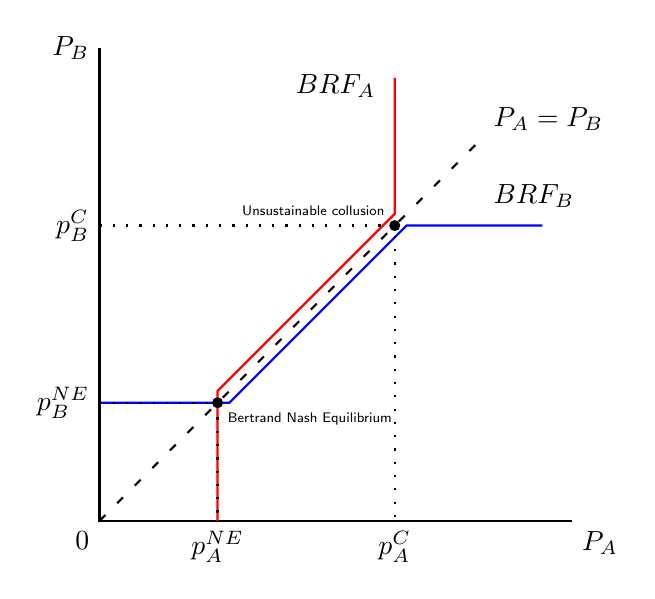
\begin{tikzpicture}[thick,font=\sffamily,scale=1.5]
	%axis
	\draw (0,4) node[left]{$P_{B}$} -- (0,0) node[below left] {$0$} 
	  -- (4,0) node[below right]{$P_{A}$}; %labels
	
	\draw [loosely dashed] plot[domain=0:3.25,smooth] (\x,\x); %SRAS1
	
	
	\draw[red] (1,0) -- (1,1.1) -- (2.5,2.6)-- (2.5,3.75); %BRF A
	
	%BFR B	 
	\draw[blue] (0,1) -- (1.1,1) -- (2.6,2.5) -- (3.75,2.5); %part 3

	 
	 %dotted lines
	 \draw[loosely dotted] (0,1) node[left]{$p^{NE}_B$} -| node[pos=0.25,below=3mm] {}
	  (1,0) node[below]{$p^{NE}_A$}; %Bertrand NE
	 \draw[loosely dotted] (0,2.5) node[left]{$p^{C}_B$} -| node[pos=0.25,below=3mm] {}
	  (2.5,0) node[below]{$p^{C}_A$}; %collusion
	  

	
	%labels
	\node[above] at (2,3.5) {$BRF_{A}$}; %BRF A label
	\node[right] at (3.25,2.75) {$BRF_{B}$}; %BRF B label
	\node[right] at (3.25,3.4) {$P_{A}=P_{B}$}; %y=x label
	
	%dots
	\node[style={fill=black,circle,inner sep=0pt,minimum size=4pt}] at (1,1) { };Bertrand NE
	\node[below right]at (1,1) {\tiny{Bertrand Nash Equilibrium}};
	\node[style={fill=black,circle,inner sep=0pt,minimum size=4pt}] at (2.5,2.5) { };SR equib
	\node[above left]at (2.5,2.5) {\tiny{Unsustainable collusion}}; %as the BRFs do not cross
	
\end{tikzpicture}
\end{document}
    \caption{The Bertrand Competition equilibrium where firms have identical (constant) marginal  costs}
    \label{fig:5}
\end{figure}
\begin{figure}[H]
    \centering
    \documentclass[class=article, crop=false]{standalone}
\usepackage{my_preamble}
\begin{document}
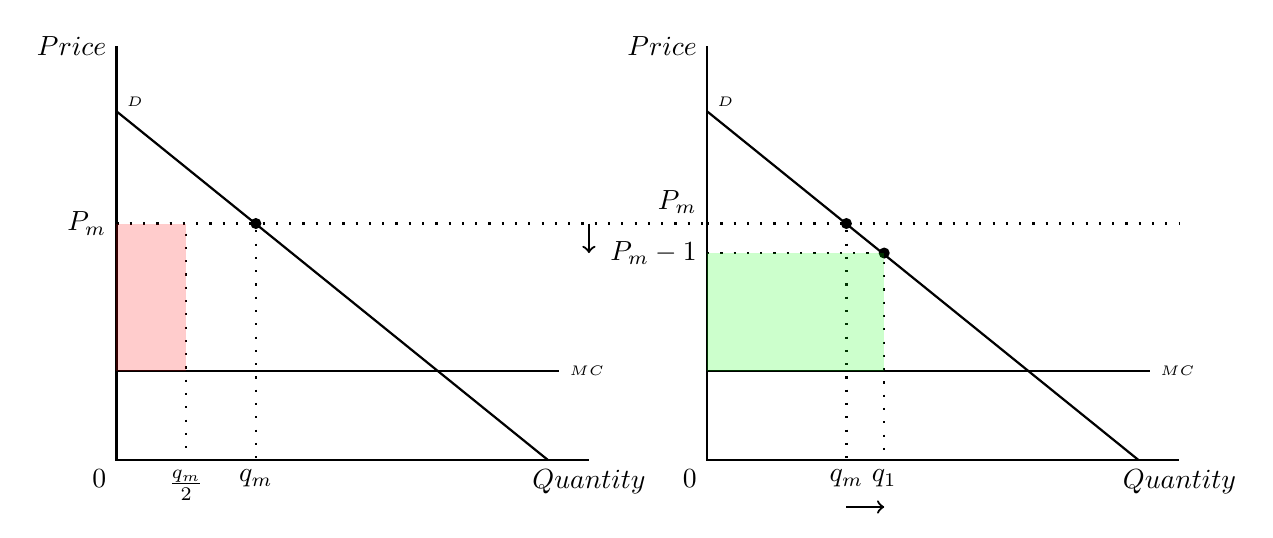
\begin{tikzpicture}[thick,font=\sffamily,scale=1.5]
	%axis
	\draw (0,3.5) node[left]{$Price$} -- (0,0) node[below left] {$0$} -- (4,0) node[below]{$Quantity$}; %graph 1
	\draw (5,3.5) node[left]{$Price$} -- (5,0) node[below left] {$0$} -- (9,0) node[below]{$Quantity$}; %graph 2
	
	%graph 1
		%curves and labels
		\draw[] (0,2.95) -- (3.65,0); %Demand
		\node[above right]at (0,2.9) {\tiny{$D$}}; %Demand label
		\draw[] (0,0.75) -- (3.75,0.75); %MC
		\node[right]at (3.75,0.75) {\tiny{$MC$}}; %MC label
		
		%nodes and dotted lines
		\draw[loosely dotted] (0,2) -- (5,2); %dotted monop price (first half)
		\draw[loosely dotted] (6.18,2) -- (9,2); %dotted monop price (second half)
		\node[style={fill=black,circle,inner sep=0pt,minimum size=4pt}] at (1.18,2) { }; %LHS node
		\draw[loosely dotted] (0,2) node[left]{$P_m$} -| node[pos=0.25,below=3mm] {}
	  (1.18,0) node[below]{$q_m$}; %Qm dotted lines
	  \draw[loosely dotted] (0,2) node[left]{} -| node[pos=0.25,below=3mm] {}
	  (0.59,0) node[below]{$\frac{q_m}{2}$}; %Qm/2 dotted lines
		
		\fill [fill=red, fill opacity=0.2] (0,2) node[left]{} -- (0.59,2) node[below left] {} -- (0.59,0.75) node[below left] {} -- (0,0.75) node[below left] {}; %fill
		
	%graph 2
		%curves and labels
		\draw[] (5,2.95) -- (8.65,0); %Demand
		\node[above right]at (5,2.9) {\tiny{$D$}}; %Demand label
		\draw[] (5,0.75) -- (8.75,0.75); %MC
		\node[right]at (8.75,0.75) {\tiny{$MC$}}; %MC label
		
		%nodes and dotted lines
		\node[style={fill=black,circle,inner sep=0pt,minimum size=4pt}] at (6.18,2) { }; %RHS node 1
		\node[style={fill=black,circle,inner sep=0pt,minimum size=4pt}] at (6.5,1.75) { }; %RHS node 2
		\draw[loosely dotted] (5,2) node[above left]{$P_m$} -| node[pos=0.25,below=3mm] {}
	  (6.18,0) node[below]{$q_m$}; %Qm dotted lines
	  \draw[loosely dotted] (5,1.75) node[left]{$P_m-1$} -| node[pos=0.25,below=3mm] {}
	  (6.5,0) node[below]{$q_1$}; %Pm-1 dotted lines
	  
		%arrows
		\draw [->] (6.18,-0.4) -- (6.5,-0.4); %x arrow
		\draw [->] (4,2) -- (4,1.75); %y arrow
  
	\fill [fill=green, fill opacity=0.2] (5,1.75) node[left]{} -- (6.5,1.75) node[below left] {} -- (6.5,0.75) node[below left] {} -- (5,0.75) node[below left] {}; %fill
  
\end{tikzpicture}
%\node[above right]at (1.8,1.5) {\tiny{$SRAS_{0}$}};
\end{document}
    \caption{Incentives to cheat under Bertrand competition}
    \label{fig:6}
\end{figure}
\begin{figure}[H]
    \centering
    \documentclass[class=article, crop=false]{standalone}
\usepackage{my_preamble}
\begin{document}
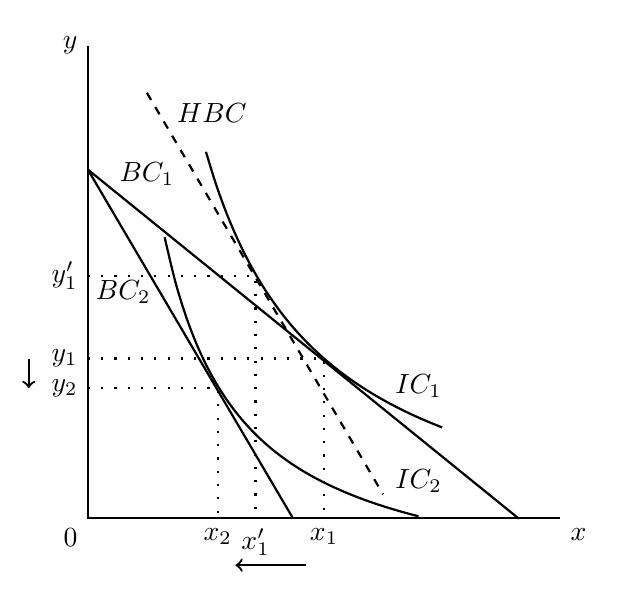
\begin{tikzpicture}[thick,font=\sffamily,scale=1.5]
	%axis
	\draw (0,4) node[left]{$y$} -- (0,0) node[below left] {$0$} -- (4,0) node[below right]{$x$}; %labels
	
	%curves
	\draw plot[domain=0:3.65,smooth] (\x,2.95-0.81*\x); %BC1
	\draw plot[domain=0:1.73,smooth] (\x,2.95-1.7*\x); %BC2
	\draw plot[domain=1:3,smooth] (\x,3.5/\x-0.4); %IC1
	\draw plot[domain=0.65:2.8,smooth] (\x,2/\x-0.7); %IC2

	%dotted lines
	\draw[loosely dotted] (0,1.35) node[left]{$y_1$} -| node[pos=0.25,below=3mm] {} (2,0) node[below]{$x_1$}; %dotted lines 1
	\draw[loosely dotted] (0,1.1) node[left]{$y_2$} -| node[pos=0.25,below=3mm] {} (1.1,0) node[below]{$x_2$}; %dotted lines 2
	
	%labels and arrows
	\node[below] at (0.5,3.1) {$BC_{1}$}; %BC1 label
	\node[below] at (0.3,2.1) {$BC_{2}$}; %BC2 label
	\node[below] at (2.8,1.3) {$IC_{1}$}; %IC1 label
	\node[below] at (2.8,0.5) {$IC_{2}$}; %IC2 label
	\draw [->] (1.85,-0.4) -- (1.25,-0.4); %x arrow
	\draw [->] (-0.5,1.35) -- (-0.5,1.1); %y arrow

	%Hypothetical
	\draw [dashed] plot[domain=0.5:2.5] (\x,4.45-1.7*\x); %BC2
	\node[below] at (1.05,3.6) {$HBC$}; %HBC label

	%CV
	\draw[loosely dotted] (0,2.05) node[left]{$y^\prime_1$} -| node[pos=0.25,below=3mm] {} (1.42,0) node[below]{$x^\prime_1$}; %dotted lines
\end{tikzpicture}
\end{document}
    \caption{Compensating variation using the Hicksian measure}
    \label{fig:7}
\end{figure}
\begin{figure}[H]
    \centering
    \documentclass[class=article, crop=false]{standalone}
\usepackage{my_preamble}
\begin{document}
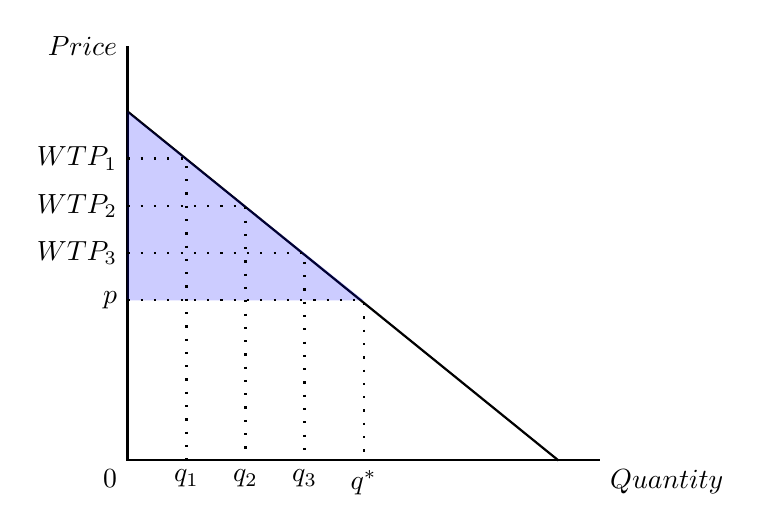
\begin{tikzpicture}[thick,font=\sffamily,scale=1.5]
 \draw (0,3.5) node[left]{$Price$} -- (0,0) node[below left] {$0$} 
  -- (4,0) node[below right]{$Quantity$}; %labels
\draw plot[domain=0:3.65,smooth] (\x,2.95-0.81*\x); %BC1
\fill [fill=blue, fill opacity=0.2] (0,2.95) node[left]{} -- (2,1.35) node[below left] {} -- (0,1.35) node[below left] {}; %fill

%dotted lines
 \draw[loosely dotted] (0,2.55) node[left]{$WTP_1$} -| node[pos=0.25,below=3mm] {}
  (0.5,0) node[below]{$q_1$}; %dotted lines
 \draw[loosely dotted] (0,2.15) node[left]{$WTP_2$} -| node[pos=0.25,below=3mm] {}
  (1,0) node[below]{$q_2$}; %dotted lines
 \draw[loosely dotted] (0,1.75) node[left]{$WTP_3$} -| node[pos=0.25,below=3mm] {}
  (1.5,0) node[below]{$q_3$}; %dotted lines
 \draw[loosely dotted] (0,1.35) node[left]{$p$} -| node[pos=0.25,below=3mm] {}
  (2,0) node[below]{$q^{*}$}; %dotted lines
\end{tikzpicture}
\end{document}
    \caption{Consumer surplus}
    \label{fig:8}
\end{figure}
\begin{figure}[H]
    \centering
    \documentclass[class=article, crop=false]{standalone}
\usepackage{my_preamble}
\usepackage{pgfplots}
\begin{document}
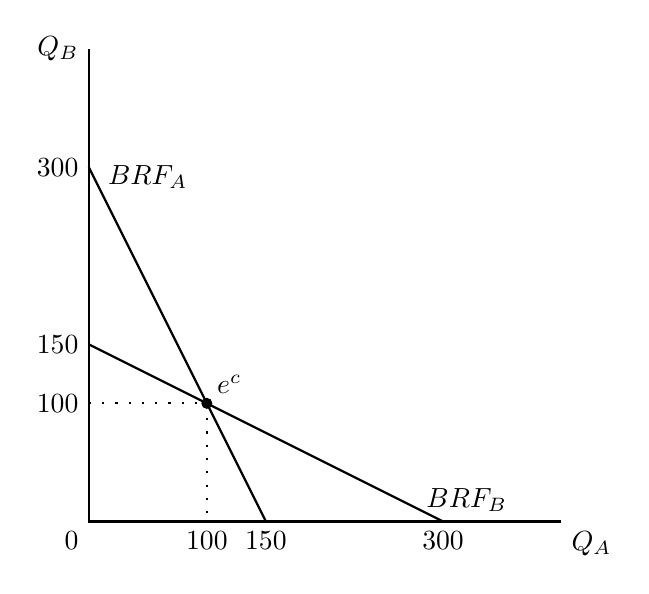
\begin{tikzpicture}[thick,font=\sffamily,scale=1.5]
	%axis
	 \draw (0,4) node[left]{$Q_{B}$} -- (0,0) node[below left] {$0$} 
	  -- (4,0) node[below right]{$Q_{A}$};
	  
	 %BRFs
	\draw[] (0,3) -- (1.5,0); %BRF A
	\draw[] (0,1.5) -- (3,0); %BRF B
	
	%labels
	\node[below] at (0.5,3.1) {$BRF_{A}$}; %BRF A label
	\node[above] at (3.2,0) {$BRF_{B}$}; %BRF B label
	\node[below] at (1.5,0) {$150$}; %A's monopoly quantity
	\node[left] at (0,1.5) {$150$}; %B's monopoly quantity
	\node[below] at (3,0) {$300$}; %PC quantity - A's???
	\node[left] at (0,3) {$300$}; %PC quantity
	
	%equilibria labels
	\node[style={fill=black,circle,inner sep=0pt,minimum size=4pt}] at (1,1) { };
	\node[above right]at (1,1) {$e^{c}$};

	%dotted lines	
	\draw[loosely dotted] (0,1) node[left]{$100$} -| node[pos=0.25,below=3mm] {}
	  (1,0) node[below]{$100$}; %cournot dotted lines
	
\end{tikzpicture}
\end{document}
    \caption{Cournot equilibrium and the outcome under collusion}
    \label{fig:9}
\end{figure}
\begin{figure}[H]
    \centering
    \documentclass[class=article, crop=false]{standalone}
\usepackage{my_preamble}
\begin{document}
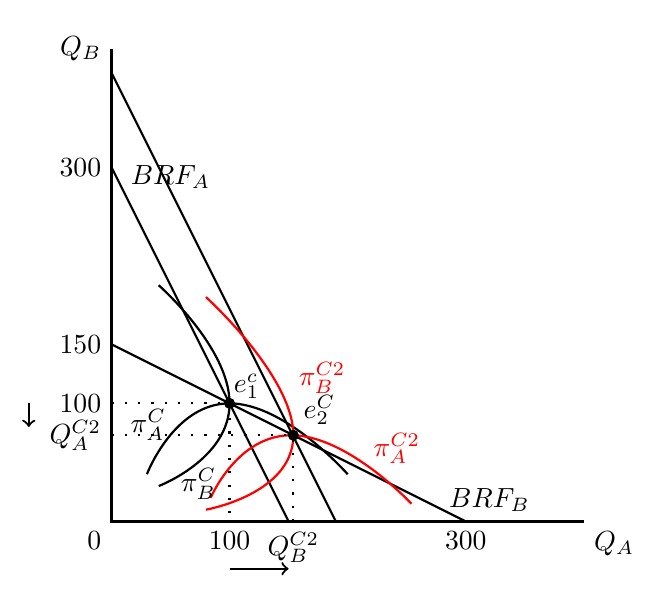
\begin{tikzpicture}[thick,font=\sffamily,scale=1.5]
	%axis
	 \draw (0,4) node[left]{$Q_{B}$} -- (0,0) node[below left] {$0$} -- (4,0) node[below right]{$Q_{A}$};
	  
	 %BRFs
	\draw[] (0,3) -- (1.5,0); %BRF A
	\draw[] (0,3.8) -- (1.9,0); %BRF A 2
	\draw[] (0,1.5) -- (3,0); %BRF B

	%Iso-profits
	\draw[] plot [smooth, tension=1] coordinates {(0.3,0.4) (1,1) (2,0.4)}; %A's iso-profit 1
	\draw[red] plot [smooth, tension=1] coordinates {(0.84,0.2) (1.54,0.73) (2.54,0.15)}; %A's iso-profit 2
	\draw[] plot [smooth, tension=1] coordinates {(0.4,0.3) (1,1) (0.4,2)}; %B's iso-profit 1
	\draw[red] plot [smooth, tension=1] coordinates {(0.8,0.1) (1.54,0.73) (0.8,1.9)}; %B's iso-profit 2
	
	%labels
	\node[below] at (0.5,3.1) {$BRF_{A}$}; %BRF A label
	\node[above] at (3.2,0) {$BRF_{B}$}; %BRF B label
	%\node[below] at (1.5,0) {$150$}; %A's monopoly quantity
	\node[left] at (0,1.5) {$150$}; %B's monopoly quantity
	\node[below] at (3,0) {$300$}; %A's PC quantity
	\node[left] at (0,3) {$300$}; %B's PC quantity
	\node[above left]at (0.55,0.6) {$\pi_A^C$}; %A's iso-profit 1 label
	\node[above right]at (0.5,0.1) {$\pi_B^C$}; %B's iso-profit 1 label
	\node[above left, red]at (2.7,0.4) {$\pi_A^{C2}$}; %A's iso-profit 2 label
	\node[above right, red]at (1.5,1) {$\pi_B^{C2}$}; %B's iso-profit 2 label
	
	
	%equilibria labels
	\node[style={fill=black,circle,inner sep=0pt,minimum size=4pt}] at (1,1) { };
	\node[above right]at (0.95,0.95) {$e^{c}_1$};
	\node[style={fill=black,circle,inner sep=0pt,minimum size=4pt}] at (1.54,0.73) { };
	\node[above right]at (1.54,0.73) {$e^{C}_2$};
	
	%dotted lines	
	\draw[loosely dotted] (0,1) node[left]{$100$} -| node[pos=0.25,below=3mm] {} (1,0) node[below]{$100$}; %cournot dotted lines
	\draw[loosely dotted] (0,0.73) node[left]{$Q^{C2}_A$} -| node[pos=0.25,below=3mm] {} (1.54,0) node[below]{$Q^{C2}_B$}; %new dotted lines
	
	%arrows
	\draw [->] (1,-0.4) -- (1.5,-0.4); %x arrow
	\draw [->] (-0.7,1) -- (-0.7,0.8); %y arrow
\end{tikzpicture}
\end{document}
    \caption{The effect of a reduction in Firm A's marginal costs on the Cournot equilibrium}
    \label{fig:10}
\end{figure}
\begin{figure}[H]
    \centering
    \documentclass[class=article, crop=false]{standalone}
\usepackage{my_preamble}
\begin{document}
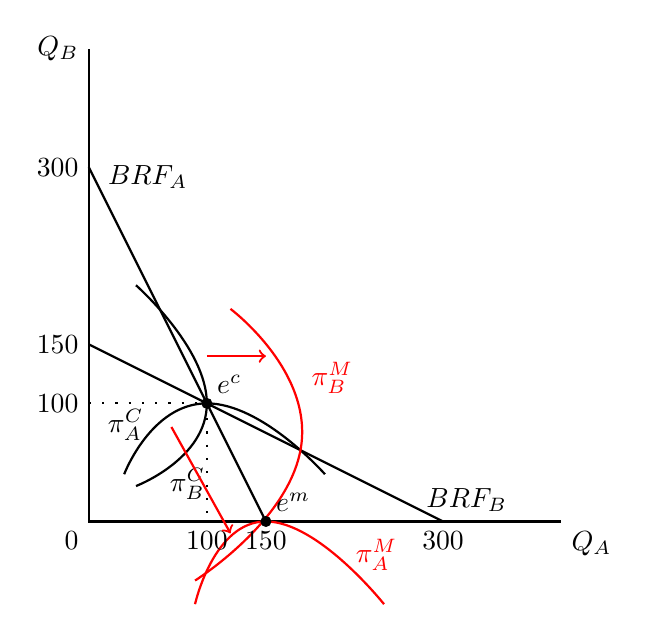
\begin{tikzpicture}[thick,font=\sffamily,scale=1.5]
	%axis
	 \draw (0,4) node[left]{$Q_{B}$} -- (0,0) node[below left] {$0$} -- (4,0) node[below right]{$Q_{A}$};
	  
	 %BRFs
	\draw[] (0,3) -- (1.5,0); %BRF A
	\draw[] (0,1.5) -- (3,0); %BRF B

	%Iso-profits
	\draw[] plot [smooth, tension=1] coordinates {(0.3,0.4) (1,1) (2,0.4)}; %A's iso-profit 1
	\draw[red] plot [smooth, tension=1] coordinates {(0.9,-0.7) (1.5,0) (2.5,-0.7)}; %A's iso-profit 2
	\draw[] plot [smooth, tension=1] coordinates {(0.4,0.3) (1,1) (0.4,2)}; %B's iso-profit 1
	\draw[red] plot [smooth, tension=1] coordinates {(0.9,-0.5) (1.8,0.65) (1.2,1.8)}; %B's iso-profit 2
	
	%labels
	\node[below] at (0.5,3.1) {$BRF_{A}$}; %BRF A label
	\node[above] at (3.2,0) {$BRF_{B}$}; %BRF B label
	\node[below] at (1.5,0) {$150$}; %A's monopoly quantity
	\node[left] at (0,1.5) {$150$}; %B's monopoly quantity
	\node[below] at (3,0) {$300$}; %A's PC quantity
	\node[left] at (0,3) {$300$}; %B's PC quantity
	\node[above left]at (0.55,0.6) {$\pi_A^C$}; %A's iso-profit 1 label
	\node[above right]at (0.6,0.1) {$\pi_B^C$}; %B's iso-profit 1 label
	\node[above left, red]at (2.7,-0.5) {$\pi_A^M$}; %A's iso-profit 2 label
	\node[above right, red]at (1.8,1) {$\pi_B^M$}; %B's iso-profit 2 label
	
	
	%equilibria labels
	\node[style={fill=black,circle,inner sep=0pt,minimum size=4pt}] at (1,1) { };
	\node[above right]at (1,1) {$e^{c}$};
	\node[style={fill=black,circle,inner sep=0pt,minimum size=4pt}] at (1.5,0) { };
	\node[above right]at (1.5,0) {$e^{m}$};
	
	%dotted lines	
	\draw[loosely dotted] (0,1) node[left]{$100$} -| node[pos=0.25,below=3mm] {}
	  (1,0) node[below]{$100$}; %cournot dotted lines
	
	%arrows
	\draw [->, red] (0.7,0.8) -- (1.2,-0.1); %A's arrow
	\draw [->, red] (1,1.4) -- (1.5,1.4); %B's arrow
\end{tikzpicture}
\end{document}
    \caption{Comparing Cournot profits to A's profits as a monopolist}
    \label{fig:11}
\end{figure}
\begin{figure}[H]
    \centering
    \documentclass[class=article, crop=false]{standalone}
\usepackage{my_preamble}
\usepackage{pgfplots}
\begin{document}
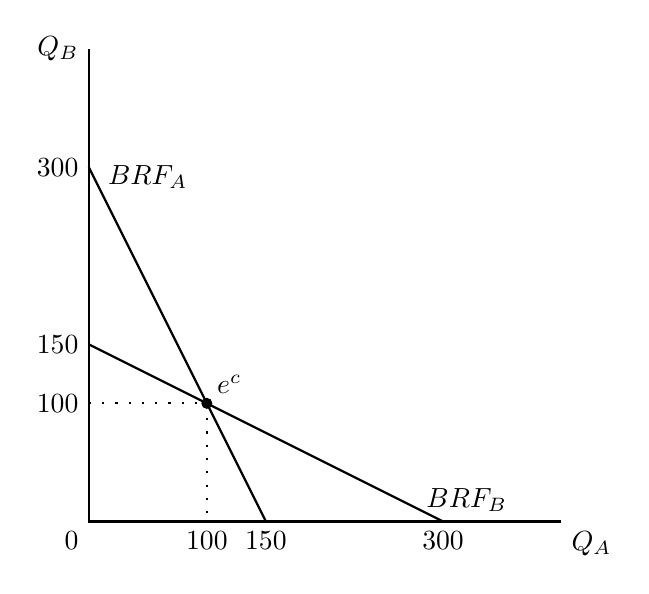
\begin{tikzpicture}[thick,font=\sffamily,scale=1.5]
	%axis
	 \draw (0,4) node[left]{$Q_{B}$} -- (0,0) node[below left] {$0$} 
	  -- (4,0) node[below right]{$Q_{A}$};
	  
	 %BRFs
	\draw[] (0,3) -- (1.5,0); %BRF A
	\draw[] (0,1.5) -- (3,0); %BRF B

	%Iso-profits
	%\draw[] plot [smooth, tension=1] coordinates {(0.3,0.4) (1,1) (2,0.4)}; %A's iso-profit 1
	%\draw[] plot [smooth, tension=1] coordinates {(0.45,0.05) (1.1,0.65) (2,0.05)}; %A's iso-profit 2
	%\draw[] plot [smooth, tension=1] coordinates {(0.4,0.3) (1,1) (0.4,2)}; %B's iso-profit 1
	%\draw[] plot [smooth, tension=1] coordinates {(0.12,0.4) (0.62,1.17) (0.05,2.05)}; %B's iso-profit 2
	
	%collusion
	%\draw[] (0.46,0.72) -- (0.75,0.5); %Contract curve	
	%\draw[] plot [smooth, tension=1] coordinates {(0.375,0.225) (1.05,0.84) (2,0.225)}; %A's iso-profit collusion
	%\draw[] plot [smooth, tension=1] coordinates {(0.26,0.35) (0.82,1.14) (0.225,2.025)}; %B's iso-profit collusion
	
	%labels
	\node[below] at (0.5,3.1) {$BRF_{A}$}; %BRF A label
	\node[above] at (3.2,0) {$BRF_{B}$}; %BRF B label
	\node[below] at (1.5,0) {$150$}; %A's monopoly quantity
	\node[left] at (0,1.5) {$150$}; %B's monopoly quantity
	\node[below] at (3,0) {$300$}; %PC quantity - A's???
	\node[left] at (0,3) {$300$}; %PC quantity
	%\node[above left]at (0.55,0.6) {$\pi_A^C$}; %A's iso-profit label
	%\node[above right]at (0.6,0.1) {$\pi_B^C$}; %B's iso-profit label
	
	
	%equilibria labels
	\node[style={fill=black,circle,inner sep=0pt,minimum size=4pt}] at (1,1) { };
	\node[above right]at (1,1) {$e^{c}$};
	%\node[style={fill=black,circle,inner sep=0pt,minimum size=4pt}] at (0.62,0.62) { };
	%\node[right]at (0.57,0.64) {\tiny{$e^{m}$}};
	
	%dotted lines	
	\draw[loosely dotted] (0,1) node[left]{$100$} -| node[pos=0.25,below=3mm] {}
	  (1,0) node[below]{$100$}; %cournot dotted lines
	%\draw[loosely dotted] (0,0.62) node[left]{$\frac{Q^{M}}{2}$} -| node[pos=0.25,below=3mm] {} (0.62,0) node[below]{$\frac{Q^{M}}{2}$}; %stackelberg dotted lines	
	
	%arrows
	%\draw [->] (1,-0.55) -- (0.63,-0.55); %x arrow
	%\draw [->] (-0.5,1) -- (-0.5,0.7); %y arrow
	%\draw [->] (0.87,1.5) -- (1.17,1.5); %B's arrow
	%\draw [->] (2.1,0.4) -- (2.1,0.25); %A's arrow
\end{tikzpicture}
\end{document}
    \caption{Best Response Functions and the Cournot equilibrium}
    \label{fig:12}
\end{figure}
\begin{figure}[H]
    \centering
    \documentclass[class=article, crop=false]{standalone}
\usepackage{my_preamble}
\usepackage{pgfplots}
\begin{document}
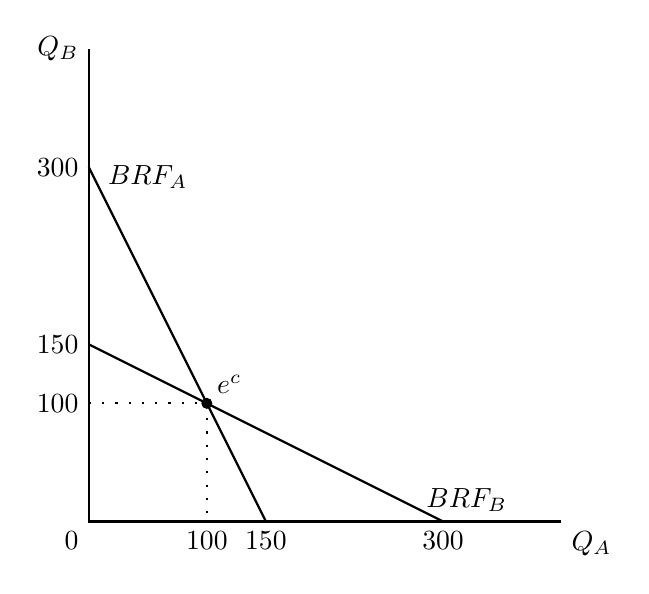
\begin{tikzpicture}[thick,font=\sffamily,scale=1.5]
	%axis
	 \draw (0,4) node[left]{$Q_{B}$} -- (0,0) node[below left] {$0$} 
	  -- (4,0) node[below right]{$Q_{A}$};
	  
	 %BRFs
	\draw[] (0,3) -- (1.5,0); %BRF A
	\draw[] (0,1.5) -- (3,0); %BRF B

	%Iso-profits
	%\draw[] plot [smooth, tension=1] coordinates {(0.3,0.4) (1,1) (2,0.4)}; %A's iso-profit 1
	%\draw[] plot [smooth, tension=1] coordinates {(0.45,0.05) (1.1,0.65) (2,0.05)}; %A's iso-profit 2
	%\draw[] plot [smooth, tension=1] coordinates {(0.4,0.3) (1,1) (0.4,2)}; %B's iso-profit 1
	%\draw[] plot [smooth, tension=1] coordinates {(0.12,0.4) (0.62,1.17) (0.05,2.05)}; %B's iso-profit 2
	
	%collusion
	%\draw[] (0.46,0.72) -- (0.75,0.5); %Contract curve	
	%\draw[] plot [smooth, tension=1] coordinates {(0.375,0.225) (1.05,0.84) (2,0.225)}; %A's iso-profit collusion
	%\draw[] plot [smooth, tension=1] coordinates {(0.26,0.35) (0.82,1.14) (0.225,2.025)}; %B's iso-profit collusion
	
	%labels
	\node[below] at (0.5,3.1) {$BRF_{A}$}; %BRF A label
	\node[above] at (3.2,0) {$BRF_{B}$}; %BRF B label
	\node[below] at (1.5,0) {$150$}; %A's monopoly quantity
	\node[left] at (0,1.5) {$150$}; %B's monopoly quantity
	\node[below] at (3,0) {$300$}; %PC quantity - A's???
	\node[left] at (0,3) {$300$}; %PC quantity
	%\node[above left]at (0.55,0.6) {$\pi_A^C$}; %A's iso-profit label
	%\node[above right]at (0.6,0.1) {$\pi_B^C$}; %B's iso-profit label
	
	
	%equilibria labels
	\node[style={fill=black,circle,inner sep=0pt,minimum size=4pt}] at (1,1) { };
	\node[above right]at (1,1) {$e^{c}$};
	%\node[style={fill=black,circle,inner sep=0pt,minimum size=4pt}] at (0.62,0.62) { };
	%\node[right]at (0.57,0.64) {\tiny{$e^{m}$}};
	
	%dotted lines	
	\draw[loosely dotted] (0,1) node[left]{$100$} -| node[pos=0.25,below=3mm] {}
	  (1,0) node[below]{$100$}; %cournot dotted lines
	%\draw[loosely dotted] (0,0.62) node[left]{$\frac{Q^{M}}{2}$} -| node[pos=0.25,below=3mm] {} (0.62,0) node[below]{$\frac{Q^{M}}{2}$}; %stackelberg dotted lines	
	
	%arrows
	%\draw [->] (1,-0.55) -- (0.63,-0.55); %x arrow
	%\draw [->] (-0.5,1) -- (-0.5,0.7); %y arrow
	%\draw [->] (0.87,1.5) -- (1.17,1.5); %B's arrow
	%\draw [->] (2.1,0.4) -- (2.1,0.25); %A's arrow
\end{tikzpicture}
\end{document}
    \caption{The efficient outcome given an endowment in an exchange economy}
    \label{fig:13}
\end{figure}
\begin{figure}[H]
    \centering
    \documentclass[class=article, crop=false]{standalone}
\usepackage{my_preamble}
\begin{document}
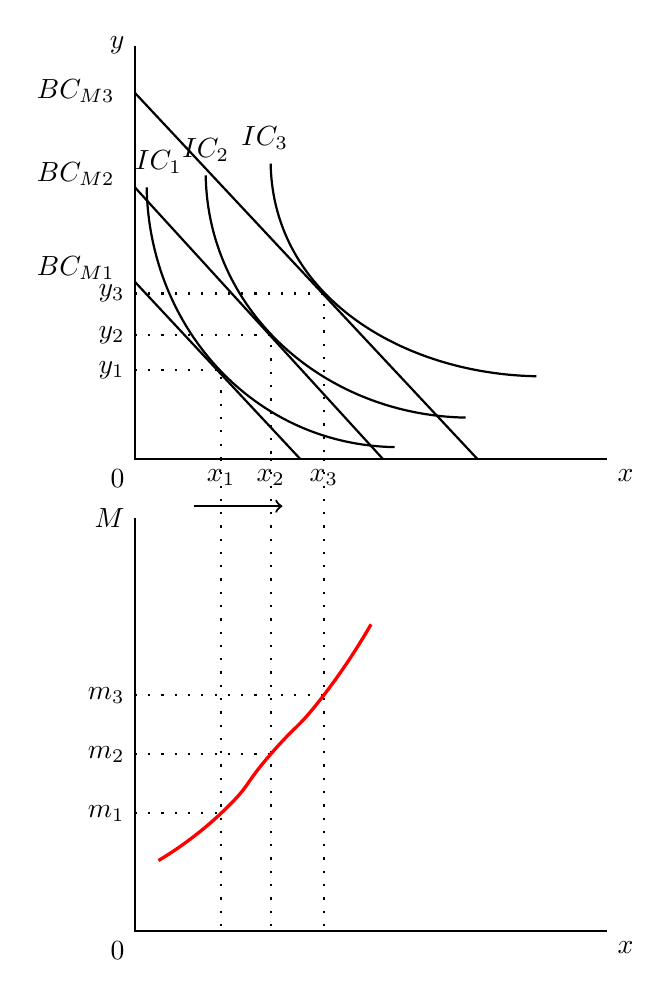
\begin{tikzpicture}[thick,font=\sffamily,scale=1.5]
%axies
 \draw (0,3.5) node[left]{$y$} -- (0,0) node[below left] {$0$} -- (4,0) node[below right]{$x$}; %top graph
 \draw (0,-0.5) node[left]{$M$} -- (0,-4) node[below left] {$0$} -- (4,-4) node[below right]{$x$}; %bottom graph
%top graph
	%equations
		%original
		\draw[] (0,1.5) -- (1.4,0); %BC1
		\draw [thick] (0.1,2.3) to [out=271,in=179] (2.2,0.1); %IC1
		
		%shift1
		\draw[] (0,2.3) -- (2.1,0); %BC2
		\draw [thick] (0.6,2.4) to [out=271,in=179] (2.8,0.35); %IC2
		
		%shift2
		\draw[] (0,3.1) -- (2.9,0); %BC3
		\draw [thick] (1.15,2.5) to [out=271,in=179] (3.4,0.7); %IC3
	
	%dotted lines
	 \draw[loosely dotted] (0,0.75) node[left]{$y_1$} -| node[pos=0.25,below=3mm] {}
	  (0.73,0) node[below]{$x_1$}; %x1 line  
	 \draw[loosely dotted] (0,1.05) node[left]{$y_2$} -| node[pos=0.25,below=3mm] {} (1.15,0) node[below]{$x_2$}; %x2 line 
	 \draw[loosely dotted] (0,1.4) node[left]{$y_3$} -| node[pos=0.25,below=3mm] {} (1.6,0) node[below]{$x_3$}; %x3 and horizontal lines
	  
	\node[below] at (-0.5,1.8) {$BC_{M1}$}; %BC label
	\node[below] at (-0.5,2.6) {$BC_{M2}$}; %BC2 label
	\node[below] at (-0.5,3.3) {$BC_{M3}$}; %BC3 label
	\node[below] at (0.2,2.7) {$IC_{1}$}; %IC1 label
	\node[below] at (0.6,2.8) {$IC_{2}$}; %IC2 label  
	\node[below] at (1.1,2.9) {$IC_{3}$}; %IC3 label
	\draw [->] (0.5,-0.4) -- (1.25,-0.4); %x arrow
	%\draw [->] (-0.5,1.35) -- (-0.5,1.1); %y arrow
%bottom graph-------------------------------
	%x Lines
	\draw[loosely dotted] (0.73,0) -- (0.73,-4); %x1
	\draw[loosely dotted] (1.15,0) -- (1.15,-4); %x2
	\draw[loosely dotted] (1.6,0) -- (1.6,-4); %x3
	
	%m lines
	\draw[loosely dotted] (0,-3) node[left]{$m_1$} -- (0.73,-3); %m1
	\draw[loosely dotted] (0,-2.5) node[left]{$m_2$} -- (1.15,-2.5); %m2
	\draw[loosely dotted] (0,-2) node[left]{$m_3$} -- (1.6,-2); %m3
	
	%Engel curve
	\draw[very thick, red] plot [smooth, tension=1] coordinates{(0.2,-3.4) (0.73,-3) (1.15,-2.5) (1.6,-2) (2,-1.4)}; %part 3
\end{tikzpicture}
\end{document}
    \caption{Deriving an Engel curve}
    \label{fig:14}
\end{figure}
\begin{figure}[H]
    \centering
    \documentclass[class=article, crop=false]{standalone}
\usepackage{my_preamble}
%Adapted from https://tex.stackexchange.com/questions/406649/drawing-a-game-tree-on-tikz/409093

\tikzset{
  % Two node styles for game trees: solid and hollow
  solid node/.style={circle,draw,inner sep=2,fill=black},
  hollow node/.style={circle,draw,inner sep=2},
  empty node/.style={rectangle,draw,fill=white,color=white}
}

% macro for entering payoffs
\newcommand\payoff[1]{
  $\begin{pmatrix} #1 \end{pmatrix}$
}

\begin{document}

\begin{tikzpicture}[every level 0 node/.style={draw,hollow node},
                   every level 1 node/.style={draw,hollow node},
                   every level 2 node/.style={draw,hollow node}, 
                   every level 3 node/.style={draw, empty node},
                   every level 4 node/.style={draw, empty node},
                   grow=right,
                   level distance=.85in,
                   sibling distance=.65in,
                   edge from parent path={(\tikzparentnode) -- (\tikzchildnode)}]
                   \tikzstyle{edge from parent}=[draw,black,very thick] 
\Tree [.\node[label=left:{{Entrant}}]{};  
        \edge node [auto=right] {1-p}; [.\node[label=left:{{Low cost}}]{}; %bottom half
			\edge node [auto=right] {}; [.\node [label=left:{Stay out}] {}; 
				\edge node [auto=right] {}; [.\node [label=left:{{Low output}}, label=right:{\payoff{0, 10}}] {};
				]
				\edge node [auto=right] {}; [.\node [label=left:{{High output}}, label=right:{\payoff{0, 12}}] {};
				]
			]
			\edge node [auto=left] {}; [.\node [label=left:{Enter}] {}; 
				\edge node [auto=right] {}; [.\node [label=left:{{Low output}}, label=right:{\payoff{4,5}}] {};
				]
				\edge node [auto=right] {}; [.\node [label=left:{{High output}}, label=right:{\payoff{-3, 6}}] {};
				]
			]
		]
        \edge node [auto=left] {p}; [.\node[label=left:{{High cost}}] {};  %top half
			\edge node [auto=right] {}; [.\node[label=left:{{Stay out}}] {}; 
				\edge node [auto=right] {}; [.\node [label=left:{{Low output}}, label=right:{\payoff{0,9}}] {};
				]
				\edge node [auto=right] {}; [.\node [label=left:{{High output}}, label=right:{\payoff{0, 8}}] {};
				]
			]
			\edge node [auto=left] {}; [.\node [label=left:{Enter}] {}; 
				\edge node [auto=right] {}; [.\node [label=left:{{Low output}}, label=right:{\payoff{4,4}}] {};
				]
				\edge node [auto=right] {}; [.\node [label=left:{{High output}}, label=right:{\payoff{-3,3}}] {};
				]
			]
		]
]
\end{tikzpicture}
\end{document}
    \caption{A vertical game tree}
    \label{fig:15}
\end{figure}
\begin{figure}[H]
    \centering
    \includestandalone[width=\textwidth]{Graphs/Market_structures.tex}
    \caption{The features of various market structures grouped by type - created with \href{https://github.com/asavagar}{Dr Anthony Savagar} and adapted from \href{https://tex.stackexchange.com/questions/78846/creating-thicker-tikz-mindmap-connectors}{this post}}
    \label{fig:16}
\end{figure}
\begin{figure}[H]
    \centering
    \documentclass[class=article, crop=false]{standalone}
\usepackage{my_preamble}
\begin{document}
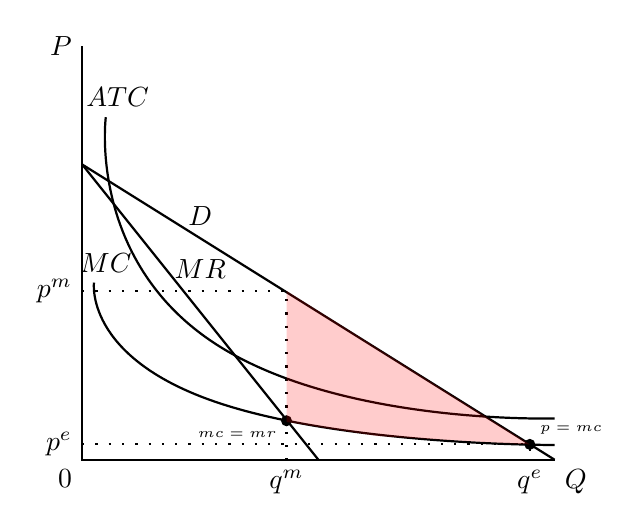
\begin{tikzpicture}[thick,font=\sffamily,scale=1.5]
	%axis
	 \draw (0,3.5) node[left]{$P$} -- (0,0) node[below left] {$0$} -- (4,0) node[below right]{$Q$};
	 
	%curves
	\draw[] (0,2.5) -- (4,0); %Demand
	\draw[] (0,2.5) -- (2,0); %MR
	\draw[] plot [smooth, tension=1] coordinates {(0.2,2.9) (1.1,1) (4,0.35)}; %ATC
	\draw[] plot [smooth, tension=1] coordinates {(0.1,1.5) (1.1,0.5) (4,0.125)}; %MC
	
	%labels
	\node[above] at (0.3,2.9) {$ATC$}; %ATC label
	\node[above] at (0.2,1.5) {$MC$}; %mC label
	\node[above] at (1,1.9) {$D$}; %D label
	\node[above] at (1,1.45) {$MR$}; %MR label
	
	%equilibria labels
	\node[style={fill=black,circle,inner sep=0pt,minimum size=4pt}] at (1.73,0.33) { }; %mc=mr node
	\node[below left]at (1.73,0.33) {\tiny{$mc=mr$}}; %mc=mr label
	\node[style={fill=black,circle,inner sep=0pt,minimum size=4pt}] at (3.79,0.13) { }; %p=mc node
	\node[above right]at (3.79,0.13) {\tiny{$p=mc$}}; %p=mc label
	
	%dotted lines	
	\draw[loosely dotted] (0,1.43) node[left]{$p^{m}$} -| node[pos=0.25,below=3mm] {}
	  (1.73,0) node[below]{$q^{m}$}; %monopoly q dotted lines
	\draw[loosely dotted] (0,0.13) node[left]{$p^{e}$} -| node[pos=0.25,below=3mm] {}
	  (3.79,0) node[below]{$q^{e}$}; %allocatively efficient dotted lines
	  
	  	\fill [fill=red, fill opacity=0.2] (1.73,1.43) node[left]{} -- (1.73,0.32) node[below left] {} -- (2.5,0.2) node[below left] {} -- (3.79,0.13) node[below left] {}; %red fill (with an intermediate coordinate to make it seem smooth)
\end{tikzpicture}
\end{document}
    \caption{The various outcomes under a natural monopoly}
    \label{fig:17}
\end{figure}
\begin{figure}[H]
    \centering
    \documentclass[class=article, crop=false]{standalone}
\usepackage{my_preamble}
\begin{document}
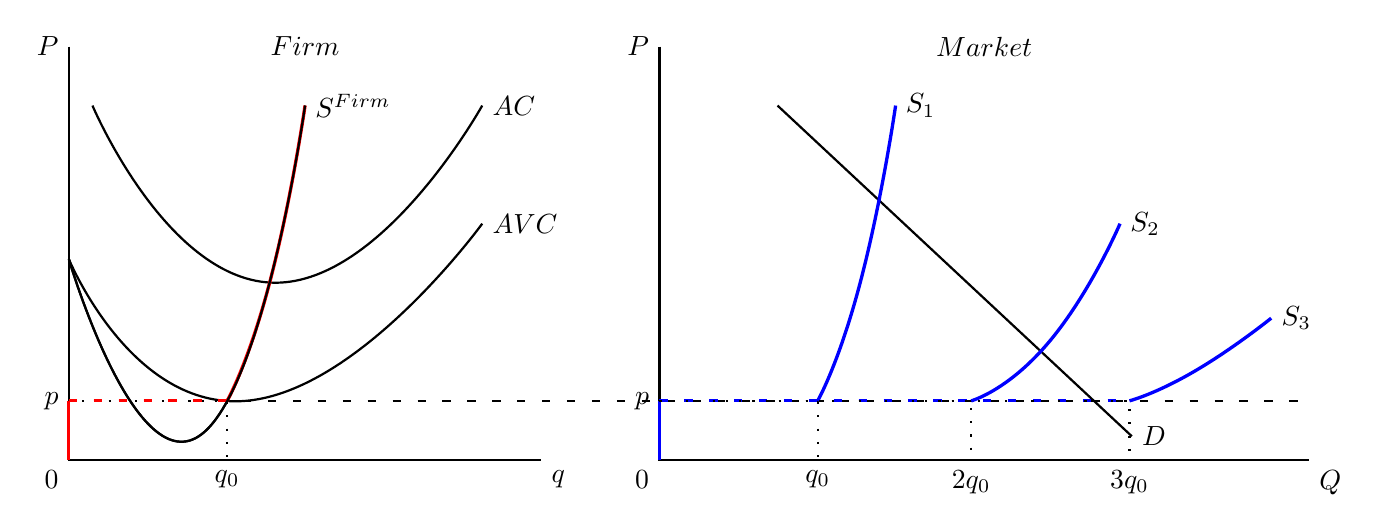
\begin{tikzpicture}[thick,font=\sffamily,scale=1.5]
	%axis and labels
	\draw (0,3.5) node[left]{$P$} -- (0,0) node[below left] {$0$} -- (4,0) node[below right]{$q$};
	\draw (5,3.5) node[left]{$P$} -- (5,0) node[below left] {$0$} -- (10.5,0) node[below right]{$Q$};
	\node[] at (2,3.5) {$Firm$}; %Firm label  
	\node[] at (7.75,3.5) {$Market$}; %Market label  
	
	%Firm--------------------------------------
		%graphs	
		\draw[] plot [smooth, tension=1] coordinates {(0.2,3) (1.75,1.5) (3.5,3)}; %AC
		\draw[] plot [smooth, tension=1] coordinates {(0,1.7) (1.5,0.5) (3.5,2)}; %AVC
		\draw[] plot [smooth, tension=1] coordinates {(0,1.7) (1.1,0.2) (2,3)}; %MC
		
		%dotted lines
		\draw[loosely dotted] (0,0.5) node[left]{$p$} -| node[pos=0.25,below=3mm] {} (1.34,0) node[below]{$q_{0}$}; %Dotted lines
		\draw[loosely dashed] (0,0.5) -- (10.5,0.5); %p line
		
		%Firm supply curve	
		\draw[very thick, red] (0,0) -- (0,0.5); %part 1
		\draw[very thick, red, loosely dashed] (0,0.5)--(1.34, 0.5); %part 2
		\draw[very thick, red] plot [smooth, tension=1] coordinates{(1.34, 0.5) (1.7,1.5) (2,3)}; %part 3
	
		%labels
		\node[right] at (2,3) {$S^{Firm}$}; %firm supply label 
		\node[right] at (3.5,3) {$AC$}; %AC label 
		\node[right] at (3.5,2) {$AVC$}; %AVC label
		\draw[] plot [smooth, tension=1] coordinates {(0,1.7) (1.1,0.2) (2,3)}; %MC
	
	%Market------------------------------------
		\draw[] (6,3) -- (9,0.2); %Demand
		
				
		%Market supply curve	
		\draw[very thick, blue] (5,0) -- (5,0.5); %part 1
		\draw[very thick, blue, loosely dashed] (5,0.5)--(9, 0.5); %part 2
		\draw[very thick, blue] plot [smooth, tension=1] coordinates{(6.34, 0.5) (6.7,1.5) (7,3)}; %part 3a
		\draw[very thick, blue] plot [smooth, tension=1] coordinates{(7.64,0.5) (8.3,1) (8.9,2)}; %part 3b
		\draw[very thick, blue] plot [smooth, tension=1] coordinates{(8.98, 0.5) (9.53,0.75) (10.18,1.2)}; %part 3c
		
		%dotted lines
		\draw[loosely dotted] (5,0.5) node[left]{$p$} -| node[pos=0.25,below=3mm] {} (6.34,0) node[below]{$q_{0}$}; %Dotted lines 1
		\draw[loosely dotted] (5,0.5) node[left]{} -| node[pos=0.25,below=3mm] {} (7.64,0) node[below]{$2q_{0}$}; %Dotted lines 2
		\draw[loosely dotted] (5,0.5) node[left]{} -| node[pos=0.25,below=3mm] {} (8.98,0) node[below]{$3q_{0}$}; %Dotted lines 3
		
		%labels
		\node[right] at (9,0.2) {$D$}; %Demand supply label  
		\node[right] at (7,3) {$S_{1}$}; %SR1 supply label  
		\node[right] at (8.9,2) {$S_{2}$}; %SR2 supply label  
		\node[right] at (10.18,1.2) {$S_{3}$}; %SR3 supply label  
\end{tikzpicture}
\end{document}
    \caption{The long run industry supply curve from a finite amount of homogeneous firms}
    \label{fig:18}
\end{figure}
\begin{figure}[H]
    \centering
    \documentclass[class=article, crop=false]{standalone}
\usepackage{my_preamble}
\begin{document}
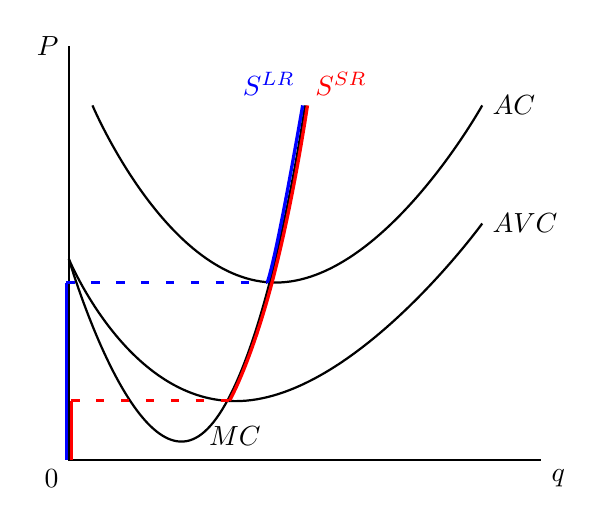
\begin{tikzpicture}[thick,font=\sffamily,scale=1.5]
	%axis and labels
	 \draw (0,3.5) node[left]{$P$} -- (0,0) node[below left] {$0$} -- (4,0) node[below right]{$q$};
	  
	%graphs	
	\draw[] plot [smooth, tension=1] coordinates {(0.2,3) (1.75,1.5) (3.5,3)}; %AC
	\draw[] plot [smooth, tension=1] coordinates {(0,1.7) (1.5,0.5) (3.5,2)}; %AVC
	\draw[] plot [smooth, tension=1] coordinates {(0,1.7) (1.1,0.2) (2,3)}; %MC
	
	%SR supply curve	
	\draw[very thick, red] (0.02,0) -- (0.02,0.5); %part 1
	\draw[very thick, red, loosely dashed] (0.02,0.5)--(1.36, 0.5); %part 2
	\draw[very thick, red] plot [smooth, tension=1] coordinates{(1.36, 0.5) (1.72,1.5) (2.02,3)}; %part 3

	%LR supply curve	
	\draw[very thick, blue] (-0.02,0) -- (-0.02,1.5); %part 1
	\draw[very thick, blue, loosely dashed] (-0.02,1.5)--(1.68, 1.5); %part 2
	\draw[very thick, blue] plot [smooth, tension=1] coordinates{(1.68,1.5) (1.795, 1.99) (1.98,3)}; %part 3

	%labelS
	\node[above right] at (2,3) {\textcolor{red}{$S^{SR}$}}; %SR supply label  
	\node[above left] at (2,3) {\textcolor{blue}{$S^{LR}$}}; %LR supply label  
	\node[right] at (3.5,3) {$AC$}; %AC label 
	\node[right] at (3.5,2) {$AVC$}; %AVC label
	\node[right] at (1.1,0.2) {$MC$}; %MC label
\end{tikzpicture}
\end{document}
    \caption{A perfectly competitive firm's supply curve in the short and long run}
    \label{fig:19}
\end{figure}
\begin{figure}[H]
    \centering
    \documentclass[class=article, crop=false]{standalone}
\usepackage{my_preamble}
\begin{document}
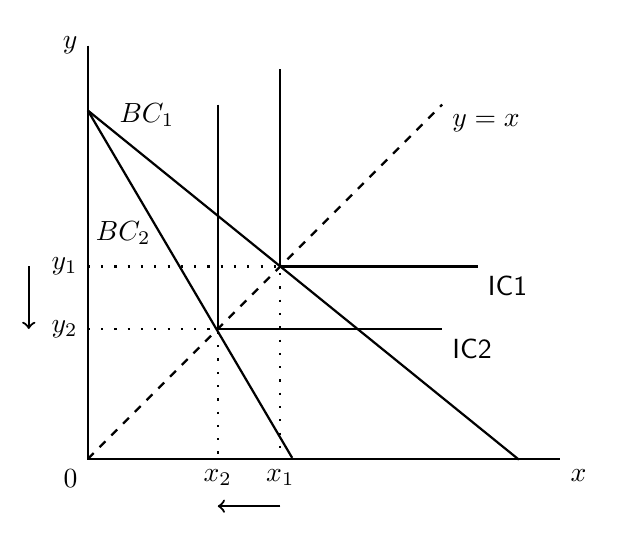
\begin{tikzpicture}[thick,font=\sffamily,scale=1.5]
	%axis
	\draw (0,3.5) node[left]{$y$} -- (0,0) node[below left] {$0$} -- (4,0) node[below right]{$x$};
	
	%graphs	
	\draw plot[domain=0:3.65,smooth] (\x,2.95-0.81*\x); %BC1
	\draw plot[domain=0:1.73,smooth] (\x,2.95-1.7*\x); %BC2
	\draw (1.63,3.3) node[left]{} -- (1.63,1.63) node[below left] {} -- (3.3,1.63) node[below right]{IC1}; %IC1
	\draw (1.1,3) node[left]{} -- (1.1,1.1) node[below left] {} 
	  -- (3,1.1) node[below right]{IC2}; %IC2
	\draw[dashed] (0,0) -- (3,3); %y=x dotted line	
	
	
	\draw[loosely dotted] (0,1.63) node[left]{$y_1$} -| node[pos=0.25,below=3mm] {} (1.63,0) node[below]{$x_1$}; %dotted lines 1
	\draw[loosely dotted] (0,1.1) node[left]{$y_2$} -| node[pos=0.25,below=3mm] {} (1.1,0) node[below]{$x_2$}; %dotted lines 2
	
	%labels and arrows
	\node[below] at (0.5,3.1) {$BC_{1}$}; %BC1 label
	\node[below] at (0.3,2.1) {$BC_{2}$}; %BC2 label
	%\node[below] at (2.8,1.3) {$IC_{1}$}; %IC1 label
	%\node[below] at (2.4,0.6) {$IC_{2}$}; %IC2 label
	\node[below right] at (3,3) {$y=x$}; %y=x label
	
	\draw [->] (1.63,-0.4) -- (1.1,-0.4); %x arrow
	\draw [->] (-0.5,1.63) -- (-0.5,1.1); %y arrow
\end{tikzpicture}
\end{document}
    \caption{Indifference curves for perfect complements}
    \label{fig:20}
\end{figure}
\begin{figure}[H]
    \centering
    \documentclass[class=article, crop=false]{standalone}
\usepackage{my_preamble}
\begin{document}
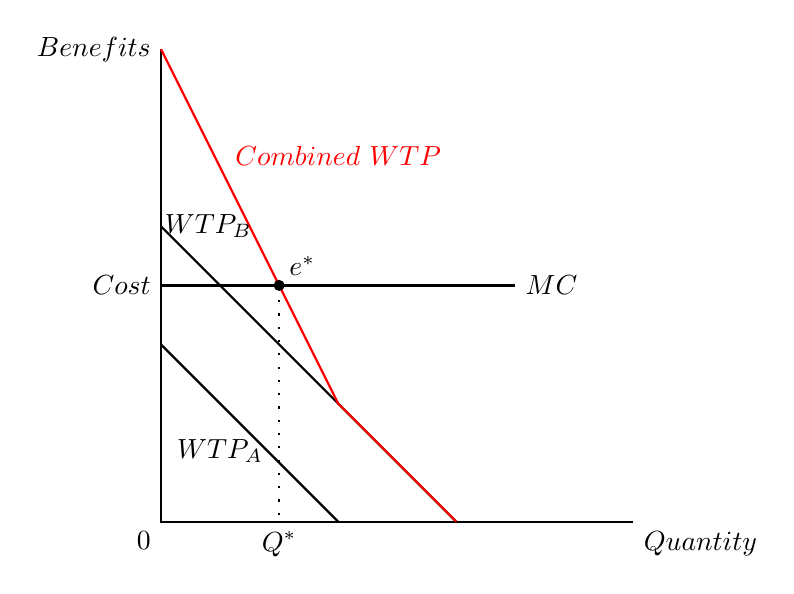
\begin{tikzpicture}[thick,font=\sffamily,scale=1.5]
	%axis
	 \draw (0,4) node[left]{$Benefits$} -- (0,0) node[below left] {$0$} 
	  -- (4,0) node[below right]{$Quantity$};
	  
	 %Graphs
	\draw[] (0,1.5) -- (1.5,0); %WTP A
	\draw[] (0,2.5) -- (2.5,0); %WTP B
	\draw[red] (0,4) -- (1.5,1) --(2.5,0); %Total WTP 
	\draw[] (0,2) -- (3,2); %MC

	
	
	%labels
	\node[red] at (1.5,3.1) {$Combined $ $WTP$}; %Total WTP label
	\node[] at (0.5,0.6) {$WTP_{A}$}; %WTP B label
	\node[] at (0.4,2.5) {$WTP_{B}$}; %WTP B label
	\node[right] at (3,2) {$MC$}; %MC label
	
	
	%equilibria labels
	\node[style={fill=black,circle,inner sep=0pt,minimum size=4pt}] at (1,2) { };
	\node[above right]at (1,2) {$e^{*}$};
	
	%dotted lines	
	\draw[loosely dotted] (0,2) node[left]{$Cost$} -| node[pos=0.25,below=3mm] {} (1,0) node[below]{$Q^{*}$}; %cournot dotted lines

\end{tikzpicture}
\end{document}
    \caption{Aggregating the agents' Willingness to Pay (WTP) for a public good}
    \label{fig:21}
\end{figure}
\begin{figure}[H]
    \centering
    \documentclass[class=article, crop=false]{standalone}
\usepackage{my_preamble}
\begin{document}
\begin{tikzpicture}[thick,font=\sffamily,scale=1.5]
	%axis
	\draw (0,3.5) node[left]{$y$} -- (0,0) node[below left] {$0$} -- (4,0) node[below right]{$x$}; %labels

	%graphs
	\draw plot[domain=0:1.1,smooth] (\x,1.87-1.7*\x); %BC1
	\draw plot[domain=0:1.47,smooth] (\x,2.5-1.7*\x); %BC2
	\draw plot[domain=0:1.87,smooth] (\x,3.2-1.7*\x); %BC3
	\draw [thick, name path = F1] (0.1,2.45) to [out=275,in=150] (1.4,0.18); %IC1
	\draw [thick, name path = F1] (0.5,2.4) to [out=275,in=160] (1.9,0.2); %IC2
	\draw [thick, name path = F1] (0.9,2.28) to [out=275,in=160] (2.37,0.18); %IC3

	%dotted lines
	\draw[loosely dotted] (0.5,1) node[left]{} -| node[pos=0.25,below=3mm] {} (0.5,0) node[below]{$x_1$}; %x1 line  
	\draw[loosely dotted] (0.85,1) node[left]{} -| node[pos=0.25,below=3mm] {} (0.88,0) node[below]{$x_2$}; %x2 line 
	\draw[loosely dotted] (0,1) node[left]{$y_1$=$y_2$=$y_3$} -| node[pos=0.25,below=3mm] {} (1.3,0) node[below]{$x_3$}; %x3 and horizontal lines
  
  %labels
	\node[below] at (-0.5,1.95) {$BC_{1}$}; %BC label
	\node[below] at (-0.5,2.6) {$BC_{2}$}; %BC2 label
	\node[below] at (-0.5,3.3) {$BC_{3}$}; %BC3 label
	\node[below] at (0.2,2.8) {$IC_{1}$}; %IC1 label
	\node[below] at (0.6,2.8) {$IC_{2}$}; %IC2 label  
	\node[below] at (1.1,2.7) {$IC_{3}$}; %IC3 label
	\draw [->] (0.5,-0.4) -- (1.25,-0.4); %x arrow
	%\draw [->] (-0.5,1.35) -- (-0.5,1.1); %y arrow
\end{tikzpicture}
\end{document}
    \caption{The effect of a change in income on quasi-linear preferences}
    \label{fig:22}
\end{figure}
\begin{figure}[H]
    \centering
    \documentclass[class=article, crop=false]{standalone}
\usepackage{my_preamble}
\begin{document}
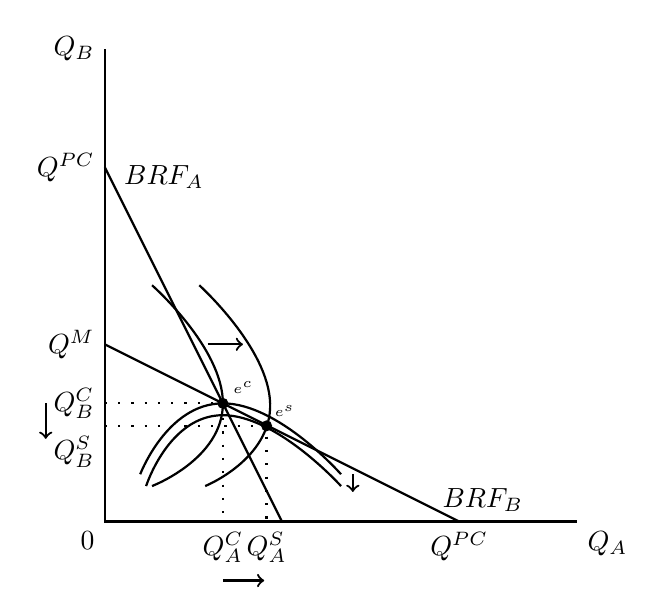
\begin{tikzpicture}[thick,font=\sffamily,scale=1.5]
	%axis
	 \draw (0,4) node[left]{$Q_{B}$} -- (0,0) node[below left] {$0$} -- (4,0) node[below right]{$Q_{A}$};
	  
	 %BRFs
	\draw[] (0,3) -- (1.5,0); %BRF A
	\draw[] (0,1.5) -- (3,0); %BRF B

	%Iso-profits
	\draw[] plot [smooth, tension=1] coordinates {(0.3,0.4) (1,1) (2,0.4)}; %A's iso-profit 1
	\draw[] plot [smooth, tension=1] coordinates {(0.35,0.3) (1,0.9) (2,0.3)}; %A's iso-profit 2
	\draw[] plot [smooth, tension=1] coordinates {(0.4,0.3) (1,1) (0.4,2)}; %B's iso-profit 1
	\draw[] plot [smooth, tension=1] coordinates {(0.85,0.3) (1.4,1) (0.8,2)}; %B's iso-profit 2
	
	%labels
	\node[below] at (0.5,3.1) {$BRF_{A}$}; %BRF A label
	\node[above] at (3.2,0) {$BRF_{B}$}; %BRF B label
	%\node[below] at (1.5,0) {$Q^{M}_A$}; %A's monopoly quantity
	\node[left] at (0,1.5) {$Q^{M}$}; %B's monopoly quantity
	\node[below] at (3,0) {$Q^{PC}$}; %PC quantity - A's???
	\node[left] at (0,3) {$Q^{PC}$}; %PC quantity
	
	%equilibria labels
	\node[style={fill=black,circle,inner sep=0pt,minimum size=4pt}] at (1,1) { };
	\node[above right]at (1,1) {\tiny{$e^{c}$}};
	\node[style={fill=black,circle,inner sep=0pt,minimum size=4pt}] at (1.37,0.81) { };
	\node[above right]at (1.35,0.8) {\tiny{$e^{s}$}};
	
	%dotted lines	
	\draw[loosely dotted] (0,1) node[left]{$Q^{C}_B$} -| node[pos=0.25,below=3mm] {}
	  (1,0) node[below]{$Q^{C}_A$}; %cournot dotted lines
	\draw[loosely dotted] (0,0.81) node[below left]{$Q^{S}_B$} -| node[pos=0.25,below=3mm] {}
	  (1.37,0) node[below]{$Q^{S}_A$}; %stackelberg dotted lines
	
	%arrows
	\draw [->] (1,-0.5) -- (1.35,-0.5); %x arrow
	\draw [->] (-0.5,1) -- (-0.5,0.7); %y arrow
	\draw [->] (0.87,1.5) -- (1.17,1.5); %A's arrow
	\draw [->] (2.1,0.4) -- (2.1,0.25); %B's arrow
\end{tikzpicture}
\end{document}
    \caption{Moving from a Cournot to Stackelberg equilibrium}
    \label{fig:23}
\end{figure}
\begin{figure}[H]
    \centering
    \documentclass[class=article, crop=false]{standalone}
\usepackage{my_preamble}
\begin{document}
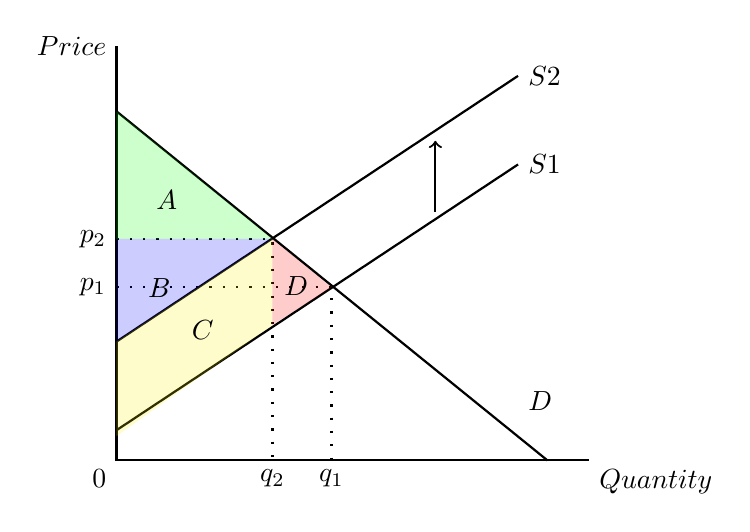
\begin{tikzpicture}[thick,font=\sffamily,scale=1.5]

	 \draw (0,3.5) node[left]{$Price$} -- (0,0) node[below left] {$0$} -- (4,0) node[below right]{$Quantity$}; %labels
	\draw plot[domain=0:3.65,smooth] (\x,2.95-0.81*\x); %Demand
	\draw[] (0,0.25) -- (3.4,2.5); %S1
	\draw[] (0,1) -- (3.4,3.25); %S2
	
	%dotted lines
	 \draw[loosely dotted] (0,1.46) node[left]{$p_{1}$} -| node[pos=0.25,below=3mm] {} (1.82,0) node[below]{$q_{1}$}; %equib 1
	 \draw[loosely dotted] (0,1.87) node[left]{$p_{2}$} -| node[pos=0.25,below=3mm] {} (1.32,0) node[below]{$q_{2}$}; %equib 2
	 
	 %fill
	\fill [fill=green, fill opacity=0.2] (0,2.95) node[left]{} -- (0,1.87) node[below left] {} -- (1.32,1.87) node[below left] {}; %green fill
	\fill [fill=blue, fill opacity=0.2] (0,1.87) node[left]{} -- (0,1) node[below left] {} -- (1.32,1.87) node[below left] {}; %blue fill
	\fill [fill=yellow, fill opacity=0.2] (0,1) node[left]{} -- (0,0.2) node[below left] {} -- (1.32,1.14) node[below left] {} -- (1.32,1.87) node[below left] {}; %yellow fill
	\fill [fill=red, fill opacity=0.2] (1.32,1.87) node[left]{} -- (1.82,1.46) node[below left] {} -- (1.32,1.14) node[below left] {}; %red fill
	
	%labels and arrows 
	\node[right] at (3.4,0.5) {$D$}; %Demand label
	\node[right] at (3.4,2.5) {$S1$}; %s1 label
	\node[right] at (3.4,3.25) {$S2$}; %s2 label
	
	\node[right] at (0.25,2.2) {$A$}; %A label
	\node[right] at (0.18,1.45) {$B$}; %B label
	\node[right] at (0.55,1.1) {$C$}; %C label
	\node[left] at (1.71,1.47) {$D$}; %D label
	 
	\draw [->] (2.7,2.1) -- (2.7,2.7); %x arrow
\end{tikzpicture}
\end{document}
    \caption{Total surplus split into multiple sections}
    \label{fig:24}
\end{figure}
\end{document}
